\documentclass{beamer}
\usetheme[numbering=fraction]{metropolis}

\usefonttheme{professionalfonts}
\setbeamercolor{background canvas}{fg=black,bg=white}

\usepackage{stix}

% \usepackage[absolute,overlay]{textpos}
% \usepackage[texcoord,
% grid,gridcolor=red!10,subgridcolor=green!10,gridunit=pt]
% {eso-pic}

\usepackage{booktabs}
\usepackage{siunitx}
\usepackage[beamer,customcolors]{hf-tikz}

\definecolor{cGreen}{HTML}{d9f4d9}
\definecolor{cRed}{HTML}{ffd9e0}
\colorlet{cGreen}{green!5}
\colorlet{cGreenD}{green!50!gray}
\colorlet{cRed}{red!5}
\colorlet{cRedD}{red!50!gray}

\colorlet{black}{black!50!gray}
\colorlet{green}{green!50!gray}
\colorlet{blue}{blue!50!gray}
\colorlet{red}{red!50!gray}

\graphicspath{{figures/}}

\title{Least-squares parameter estimation in the presence of outliers}
\author{Dmitry I.~Kabanov}
\institute{RWTH Aachen University}
\date{Book chapter presentations on Stochastic Numerics\\17 June 2019}
%\logo{\vspace{-1cm}
\includegraphics[scale=0.8]{RWTH-logo.pdf}}
\titlegraphic{%
    \begin{picture}(12.8,9.6)
    \put(-11,-230){
\includegraphics[scale=0.8]{RWTH-logo.pdf}}
    \end{picture}
}

\usepackage{amsmath}

% --- Macros
\newcommand{\R}{{\mathbb R}}
\renewcommand{\vec}{\boldsymbol}

\newcommand{\data}{\vec D}
\newcommand{\param}{\vec\theta}

\renewcommand{\Pr}[1]{\mathbb P \left(#1\right) }

\newcommand{\argmax}{\mathop{\mathrm{argmax}}}
\newcommand{\dd}{\mathrm{d}}

\setlength{\unitlength}{1cm}

\begin{document}
\begin{frame}[plain]
\titlepage
\end{frame}

% Remove logo from all other slides.
\logo{}

\begin{frame}
    \frametitle{Motivation}
    \begin{itemize}
        \item{Least-squares regression is ubiquitously used procedure
              for~parameter estimation}
        \item{However, it treats all data observations equally}
        \item Therefore, outliers get the same weight as correct data
        \item Often leads to incorrect estimates
    \end{itemize}

\end{frame}

\begin{frame}
    \frametitle{Problem setup}
    Given data \[\vec D = \{D_k\} = \{x_k, Y_k\}, \quad k = 1, \dots, N,\]
    estimate parameter $\vec\theta \in \R^M$ of the data model
    \[
        Y_k = f(x_k; \vec\theta) + \epsilon_k,
    \]
    where $f(x_k; \vec\theta)$ is ideal noiseless data and $\epsilon \in \R^N$
    is observation noise.
\end{frame}

\frame{
\frametitle{Ordinary Least Squares in Bayesian setting}
We reformulate the above problem using Bayes' theorem:
\[
    \Pr{\param | \data} \propto \Pr{\data | \param} \times \Pr{\param}
\]

\pause
\vspace{5pt}
\textbf{Assumption 1}: Uniform prior $\Pr{\param} = \text{constant}$\\
\textbf{Assumption 2}: Independent Gaussians for each datum. Then the likelihood: 
\[\Pr{\data | \param} = 
    \prod_{k=1}^N \frac{1}{\sigma_k \sqrt{2\pi}}
    \exp \left(-\frac{R_k^2}{2} \right)
    \propto 
    \exp \left(-\frac{\chi^2}{2} \right)
\]
\[
    \chi^2 = \sum_{k=1}^N R_k^2, \quad R_k = \frac{f(x_k; \param)-Y_k}{\sigma_k}
\]

\pause
The goal is to maximize log-likelihood:
\[
    \param = \argmax \left( \text{const} - \frac{\chi^2}{2} \right)
\]
}

\begin{frame}{Extension 1: conservative formulation}
Tolerate that the noise can be above some prescribed threshold:
\[
    \Pr{\sigma | \sigma_0} = \frac{\sigma_0}{\sigma^2} 
    \text{ for } \sigma\geq\sigma_0
    \text{ and zero otherwise}   
\]

Then the marginal likelihood for datum $D_k$ is:
\[
    \Pr{D_k|\sigma_0} = 
    \int_0^\infty \Pr{D_k | \sigma} \Pr{\sigma | \sigma_0} \, \dd \sigma
\]
which gives
\begin{multline*}
    \Pr{D_k | \sigma_0} = \int_0^\infty
    \frac{\sigma_0}{\sigma^3\sqrt{2\pi}}
    \exp\left( - \frac{ \left( F_k-D_k \right)^2}{2\sigma^2} \right)
    \, \dd \sigma =\\
    \frac{1}{\sigma_0 \sqrt{2\pi}} \frac{1-\exp\left( -R_k^2/2 \right)}{R_k^2}
\end{multline*}
\end{frame}


\begin{frame}{Extension 1: conservative formulation, cont.}
\begin{picture}(12.8, 9.6)
\put(0, 8.5){
\begin{minipage}{\linewidth}{
    Ordinary Least Squares: $P \sim \exp \left(- R^2/2\right)$ as $R\to\infty$\\
    Conservative formulation: $P \sim \frac{1}{R^2}$ as $R\to\infty$
    (less skewing effect)
}
\end{minipage}
}
\put(0, 1.50){
\centering
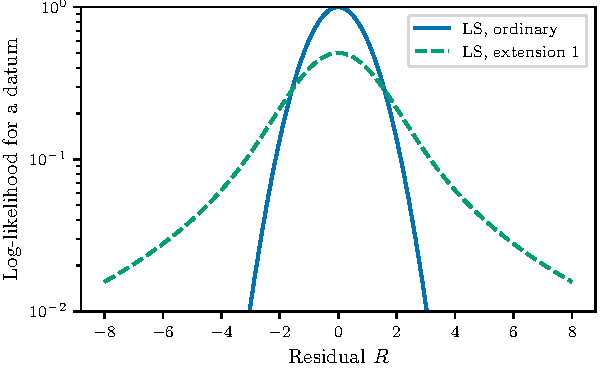
\includegraphics{likelihood-vs-residual.pdf}
}
\end{picture}
\end{frame}


\begin{frame}{Extension 1: conservative formulation, cont.}
Treat all measurements independent of each other.

Use uniform prior distribution as in Ordinary Least Squares.

\vspace{1cm}
Then log-likelihood is
\[
        \mathcal L = \ln \left(\Pr{\param | \data} \right) =
        \text{constant} + \sum_{k=1}^N \ln \left( 
            \frac{1-\exp\left( -\frac{R^2}{2}\right)}{R^2}
        \right)
\]

\pause
\vspace{1cm}
\textbf{Disadvantage}: uncertainties are worse, then for ordinary
least squares (to be seen later).
\end{frame}

\begin{frame}
\frametitle{Extension 2: the good-and-bad data model}
Distribution of noise admits two possibilities:
either noise is {\color{green}within threshold}
or it is {\color{red}very large}:

\[
    \Pr{\sigma_k | \sigma_0} = \ \ 
    \tikzmarkin<1->[set fill color=cGreen,set border color=cGreenD]{good}%
    (0.1,-0.3)(-0.1,0.5)
    (1 - \beta) \, \delta(\sigma - \sigma_0)
    \tikzmarkend{good}
    \ \   + \ \  
    \tikzmarkin<1->[set fill color=cRed,set border color=cRedD]{bad}%
    (0.1,-0.3)(-0.1,0.5)
    \beta \, \delta(\sigma - \gamma \sigma_0)
    \tikzmarkend{bad}
\]
where $0 \leq \beta \ll 1$ and $\gamma \gg 1$, $\delta(\cdot)$ the Dirac delta.

\vspace{0.5cm}
$\beta$ is the frequency of occurence of the outliers\\
$\gamma$ is the scale of the outliers

%%%%%% FIX ME: Absolute positioning!
\begin{tikzpicture}[remember picture, overlay]
\href{https://doi.org/10.1093/biomet/55.1.119}{Box\&Tiao, 1968}
\end{tikzpicture}
\end{frame}

\begin{frame}{Extension 2: the good-and-bad data model, cont.}
Treat all measurements independent of each other.

Use uniform prior distribution as in Ordinary Least Squares.

Then the log-likelihood is:
\[
    L = \text{constant} + \sum_{k=1}^N \ln \left[ 
        \frac{\beta}{\gamma} \exp \left(-\frac{R_k^2}{2\gamma^2} \right) +
        \left(1 - \beta \right) \exp \left(-\frac{R_k^2}{2} \right)
\right]
\]
where
\[
    R_k = \frac{f(x_k; \param) - Y_k}{\sigma_0}
\]
\end{frame}

\begin{frame}{Example 1: no outliers}
\begin{picture}(12.8, 9.6)
\put(0, 8.3){
\begin{minipage}{\linewidth}{
\[
    \text{31 observations:} \quad \text{data} = m x + b + 10N(0, 1)
\]
}
\end{minipage}
}
\put(0, 1.75){
\centering
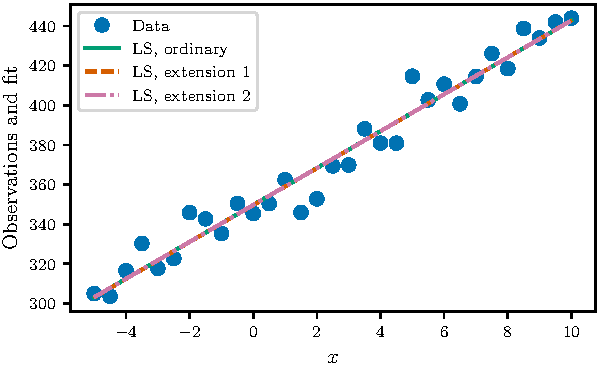
\includegraphics{good-data.pdf}
}
\end{picture}
\end{frame}

\begin{frame}{Example 1: no outliers, cont.}
\begin{picture}(12.8, 9.6)
\put(0, 8.3){
\begin{minipage}{\linewidth}{
\[
    \text{31 observations:} \quad \text{data} = m x + b + 10N(0, 1)
\]
}
\end{minipage}
}
\put(0, 1.75){
\centering
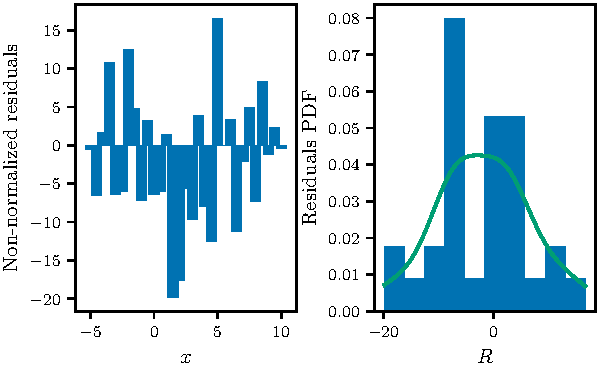
\includegraphics{residuals-good-data.pdf}
}
\end{picture}
\end{frame}

\begin{frame}{Example 1: no outliers, cont.}
\begin{picture}(12.8, 9.6)
\put(0, 8.3){
\begin{minipage}{\linewidth}{
\[
    \text{31 observations:} \quad \text{data} = m x + b + 10N(0, 1)
\]
}
\end{minipage}
}
\put(1.5, 5.75){
\centering
\begin{tabular}{lSSSS}
\toprule
Type of method & $m$ & $\text{se}_m$ & $b$ & $\text{se}_b$ \\
\midrule
Ideal & 10.0 & 0 & 350.0 & 0 \\
LS, ordinary    &  9.3 & 0.8 & 349.7 & 4.0 \\
LS, extension 1 &  9.3 & 1.2 & 349.7 & 6.2 \\
LS, extension 2 &  9.3 & 0.8 & 349.7 & 4.1 \\
\bottomrule
\end{tabular}
}
\end{picture}
\end{frame}

\begin{frame}{Example 2: six outliers}
\begin{picture}(12.8, 9.6)
\put(0, 8.3){
\begin{minipage}{\linewidth}{
\[
    \text{31 observations:} \quad \text{data} = m x + b + 10N(0, 1)
\]
\vspace{-0.75cm}
\[
    \text{6 observations are increased $2$--$5$ times}
\]
}
\end{minipage}
}
\put(0, 1.75){
\centering
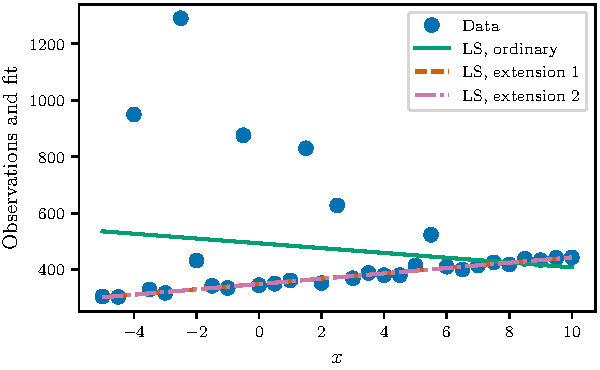
\includegraphics{bad-data.pdf}
}
\end{picture}
\end{frame}

\begin{frame}{Example 2: six outliers, cont.}
\begin{picture}(12.8, 9.6)
\put(0, 8.3){
\begin{minipage}{\linewidth}{
\[
    \text{31 observations:} \quad \text{data} = m x + b + 10N(0, 1)
\]
\vspace{-0.75cm}
\[
    \text{6 observations are increased $2$--$5$ times}
\]
}
\end{minipage}
}
\put(0, 1.75){
\centering
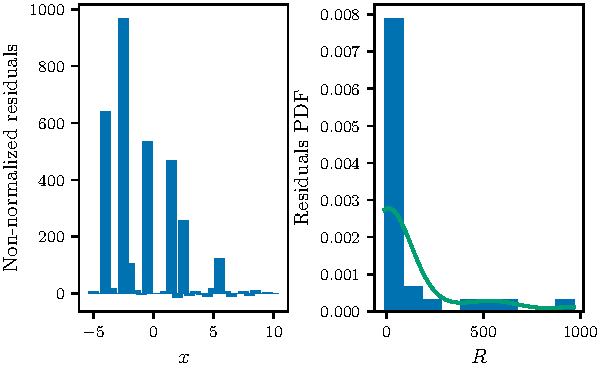
\includegraphics{residuals-bad-data.pdf}
}
\end{picture}
\end{frame}

\begin{frame}{Example 2: six outliers, cont.}
\begin{picture}(12.8, 9.6)
\put(0, 8.3){
\begin{minipage}{\linewidth}{
\[
    \text{31 observations:} \quad \text{data} = m x + b + 10N(0, 1)
\]
\vspace{-0.75cm}
\[
    \text{6 observations are increased $2$--$5$ times}
\]
}
\end{minipage}
}
\put(1.5, 5.75){
\centering
\begin{tabular}{lSSSS}
\toprule
Type of method & $m$ & $\text{se}_m$ & $b$ & $\text{se}_b$ \\
\midrule
Ideal & 10.0 & 0 & 350.0 & 0 \\
LS, ordinary    &  {\color{red}-8.5} & 0.8 & 493.5 & 4.0 \\
LS, extension 1 &  9.4 & 1.3 & 349.8 & 7.4 \\
LS, extension 2 &  9.4 & 0.9 & 349.3 & 4.9 \\
\bottomrule
\end{tabular}
}
\end{picture}
\end{frame}

\begin{frame}
{LS extension 2 has disadvantage: sensitive to parameters}
\vspace{1cm}
\centering
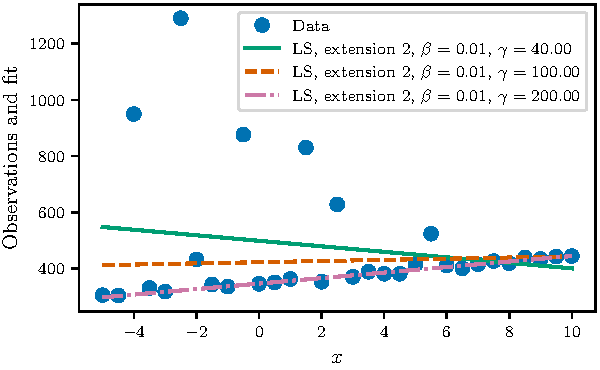
\includegraphics{fig-model-bad-and-good.pdf}
\end{frame}

\begin{frame}
{LS extension 2 has disadvantage: sensitive to parameters}
\centering
\begin{tabular}{lSSSS}
\toprule
Type of method & $m$ & $\text{se}_m$ & $b$ & $\text{se}_b$ \\
\midrule
Ideal & 10.0 & 0 & 350.0 & 0 \\
LS, ext.\ 2, $\beta = 0.01$, $\gamma = 50$ & -9.8 & 1.9 & 498.4 & 14.9 \\
LS, ext.\ 2, $\beta = 0.01$, $\gamma = 100$ & 2.1 & 1.7 & 422.2 & 15.6 \\
LS, ext.\ 2, $\beta = 0.01$, $\gamma = 200$ & 9.8 & 0.1 & 346.1 & 1.0 \\
\bottomrule
\end{tabular}
\end{frame}

\begin{frame}{Conclusions}
\begin{itemize}
    \item Ordinary Least Squares (OLS) are prone to wrong estimation 
    in~the presence of outliers (not robust)
    \item Bayesian formulation of the least-squares algorithms simplifies
    adjustments needed to accommodate outliers
    \item Two extensions were considered: conservative formulation and
    bad-and-good formulation
    \item Both formulations require careful choice of parameters for good
    performance
    \item Conservative formulation gives worse uncertainties on the estimates,
    but requires less parameters than the bad-and-good formulation
\end{itemize}
\end{frame}


\begin{frame}{References and codes}
\begin{itemize}
    \item Sivia D.\ S., Skilling J. \emph{Data analysis: a Bayesian tutorial},
    OUP Oxford, 2006
    \item Box, George E.\ P, Tiao G.\ C.
    \emph{A Bayesian approach to some outlier problems},
    Biometrika, 1968, pp.\ 119--129
    \item Codes for this presentation are available at: 
    \url{https://github.com/dmitry-kabanov/stochastic-numerics-2019-robust-least-squares}
\end{itemize}
\end{frame}

\begin{frame}[standout]
\Huge
Thank you!
\end{frame}

\end{document}